
\section{Approach}


\subsection{The Data}

The data is not given as a classic table and therefor not directly
useable for classification. It consists of two sets of images. The
first one contains the original images of each cross section and a
corresponding mask. A mask is a grayscale image with only black or
white pixels. A pixel is white if it belongs to the cross section
and black if it does not. There are $762$ images with a resolution
of $3272\times2469$, resulting in a huge amount of pixels.

\begin{lstlisting}[caption=libsvm format,label=lisbsvm] 
<class_label> <feature_id>:value ... <feature_id>:value
<class_label> <feature_id>:value ... <feature_id>:value ... 
\end{lstlisting} 

The classification problem is a binary one since there are only two
classes. Before a classifier can be trained, the images have to be
converted into a attribute value format. The libsvm format was chosen,
because it is well known and many libraries support it. Every row
represents one instance, which is in this case one pixel and its features.
Currently the only features available are the rgb values of a pixel
from the original image and the class label from the mask. 


\subsection{Data Preparation}

In the first preprocessing step the libsvm data is created. The easiest
method saves for each pixel the rgb values and the class label. This
is done for every image resulting in $762$ files. Every file has
$8.078.568$ instances, so there are $6.155.868.816$ pixels in total.
A first trivial approach took about 3 days to generate all attribute
value files.

Building a model on this set would take a huge amount of time and
is therefor unreasonable for selecting a model. Instead of using the
complete data set samples have to be used. As figure \ref{fig:mask603}
shows there are more instances of class $0$ (black pixels) than of
class $1$ (white pixels). To weight both classes equally, the sampled
set is balanced. 

\begin{figure}	
\centering 	
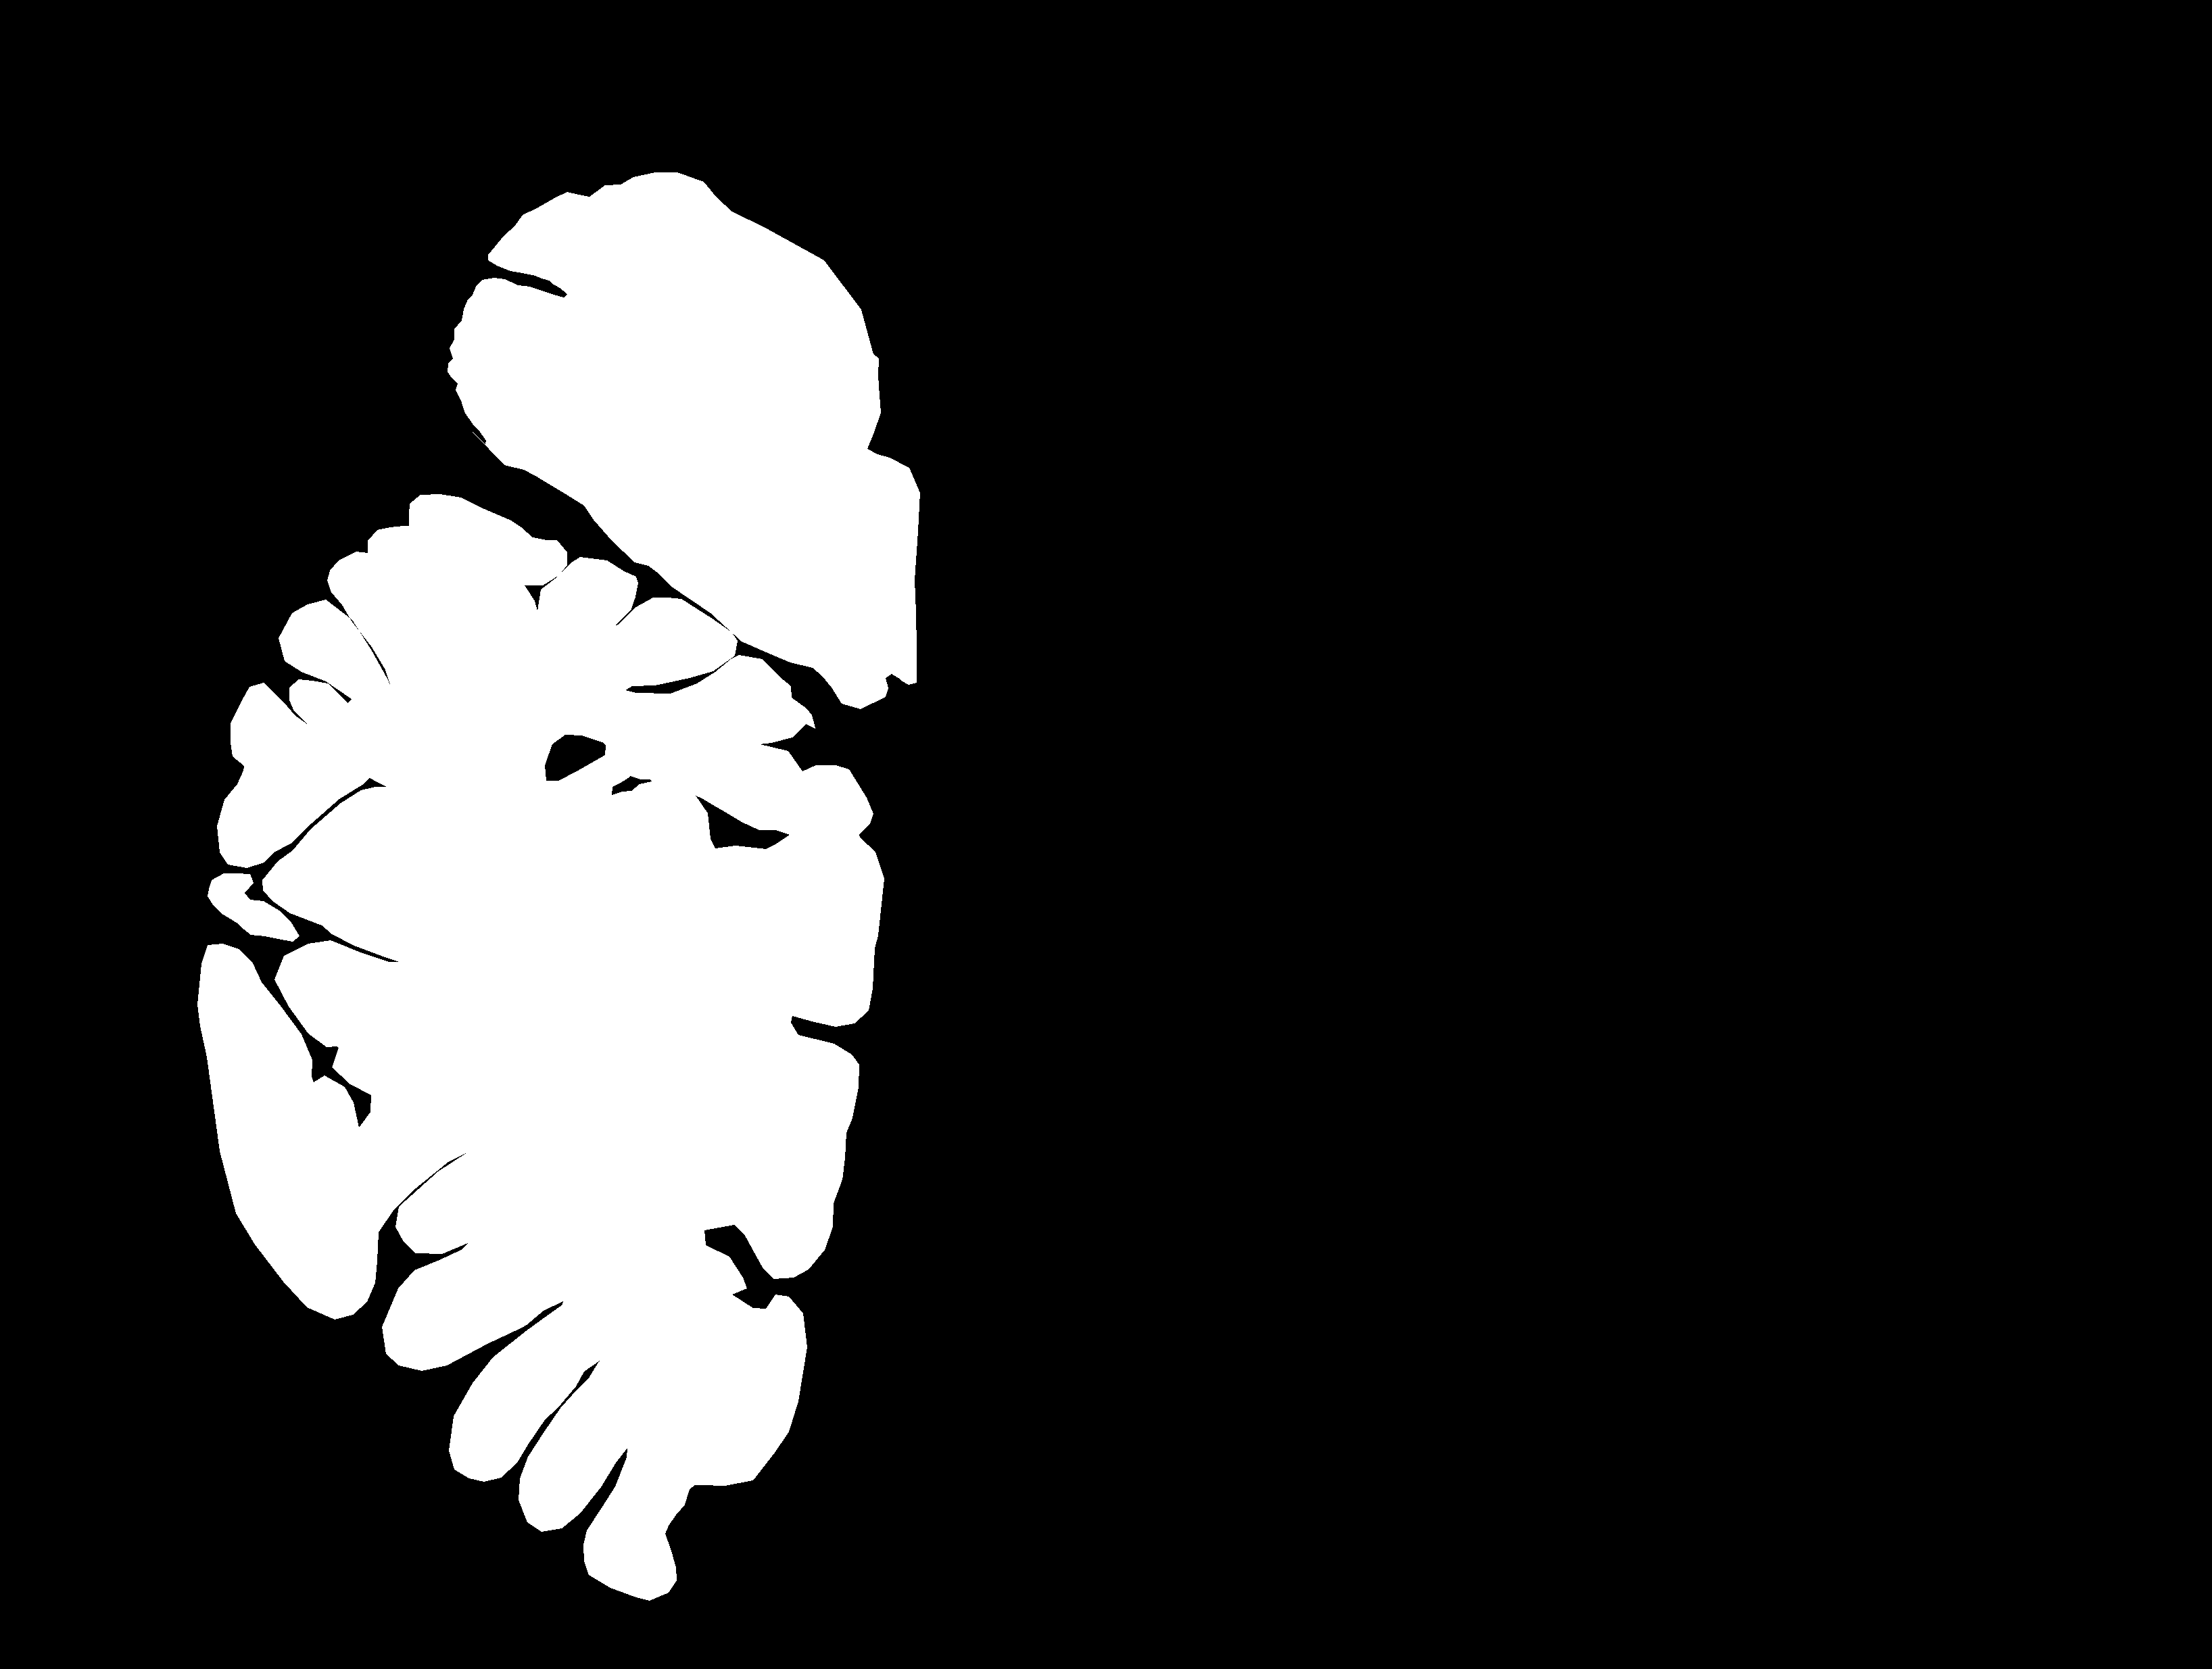
\includegraphics[width=0.6\linewidth]{graphics/mask603} 	
\caption{Mask of a cross section} 	
\label{fig:mask603} 
\end{figure}

The first approach is a balanced random sampling method. For a given
percentage $p$ and a data set with \$N\$ instances the method draws
$p\cdot N$ samples from a file. If the sample is balanced, $p\cdot N\cdot0.5$
instances of each class are drawn randomly. This can easily be parallelized
since the files can be sampled independently. This yields a first
sample with three features. To improve the classifier the number of
features has to be increased.


\subsubsection{HSV color space}

An easy method to increase the number of features is to use another
color space in addition to the given RGB values. In this case the
HSV color space was chosen. It represents a color by its hue, saturation
and value. The values for a pixel can easily be transformed from RGB
to HSV with the following formula:

\begin{eqnarray*}
Max & = & max(R,G,B)\\
Min & = & min(R,G,B)\\
H & = & \begin{cases}
0, & \text{if Max =Min \ensuremath{\Leftrightarrow}}R=G=B\\
60\text{\textdegree}\cdot\left(0+\frac{G-B}{Max-Min}\right) & \text{if Max =R }\\
60\text{\textdegree}\cdot\left(2+\frac{B-R}{Max-Min}\right) & \text{if Max =G}\\
60\text{\textdegree}\cdot\left(4+\frac{R-G}{Max-Min}\right) & \text{if Max =B}
\end{cases}\\
S & = & \begin{cases}
0 & \text{if Max =0 \ensuremath{\Leftrightarrow}R=G=B=0 }\\
\frac{Max-Min}{Max} & else
\end{cases}\\
V & = & Max
\end{eqnarray*}


Since this computation can be done independently for every pixel,
the features can easily be computed in parallel and be added to existing
data. While computing the HSV values is simple, they also add only
few additional information. Because of this the increase of accuracy
is only marginal.

\begin{figure} 
\centering 
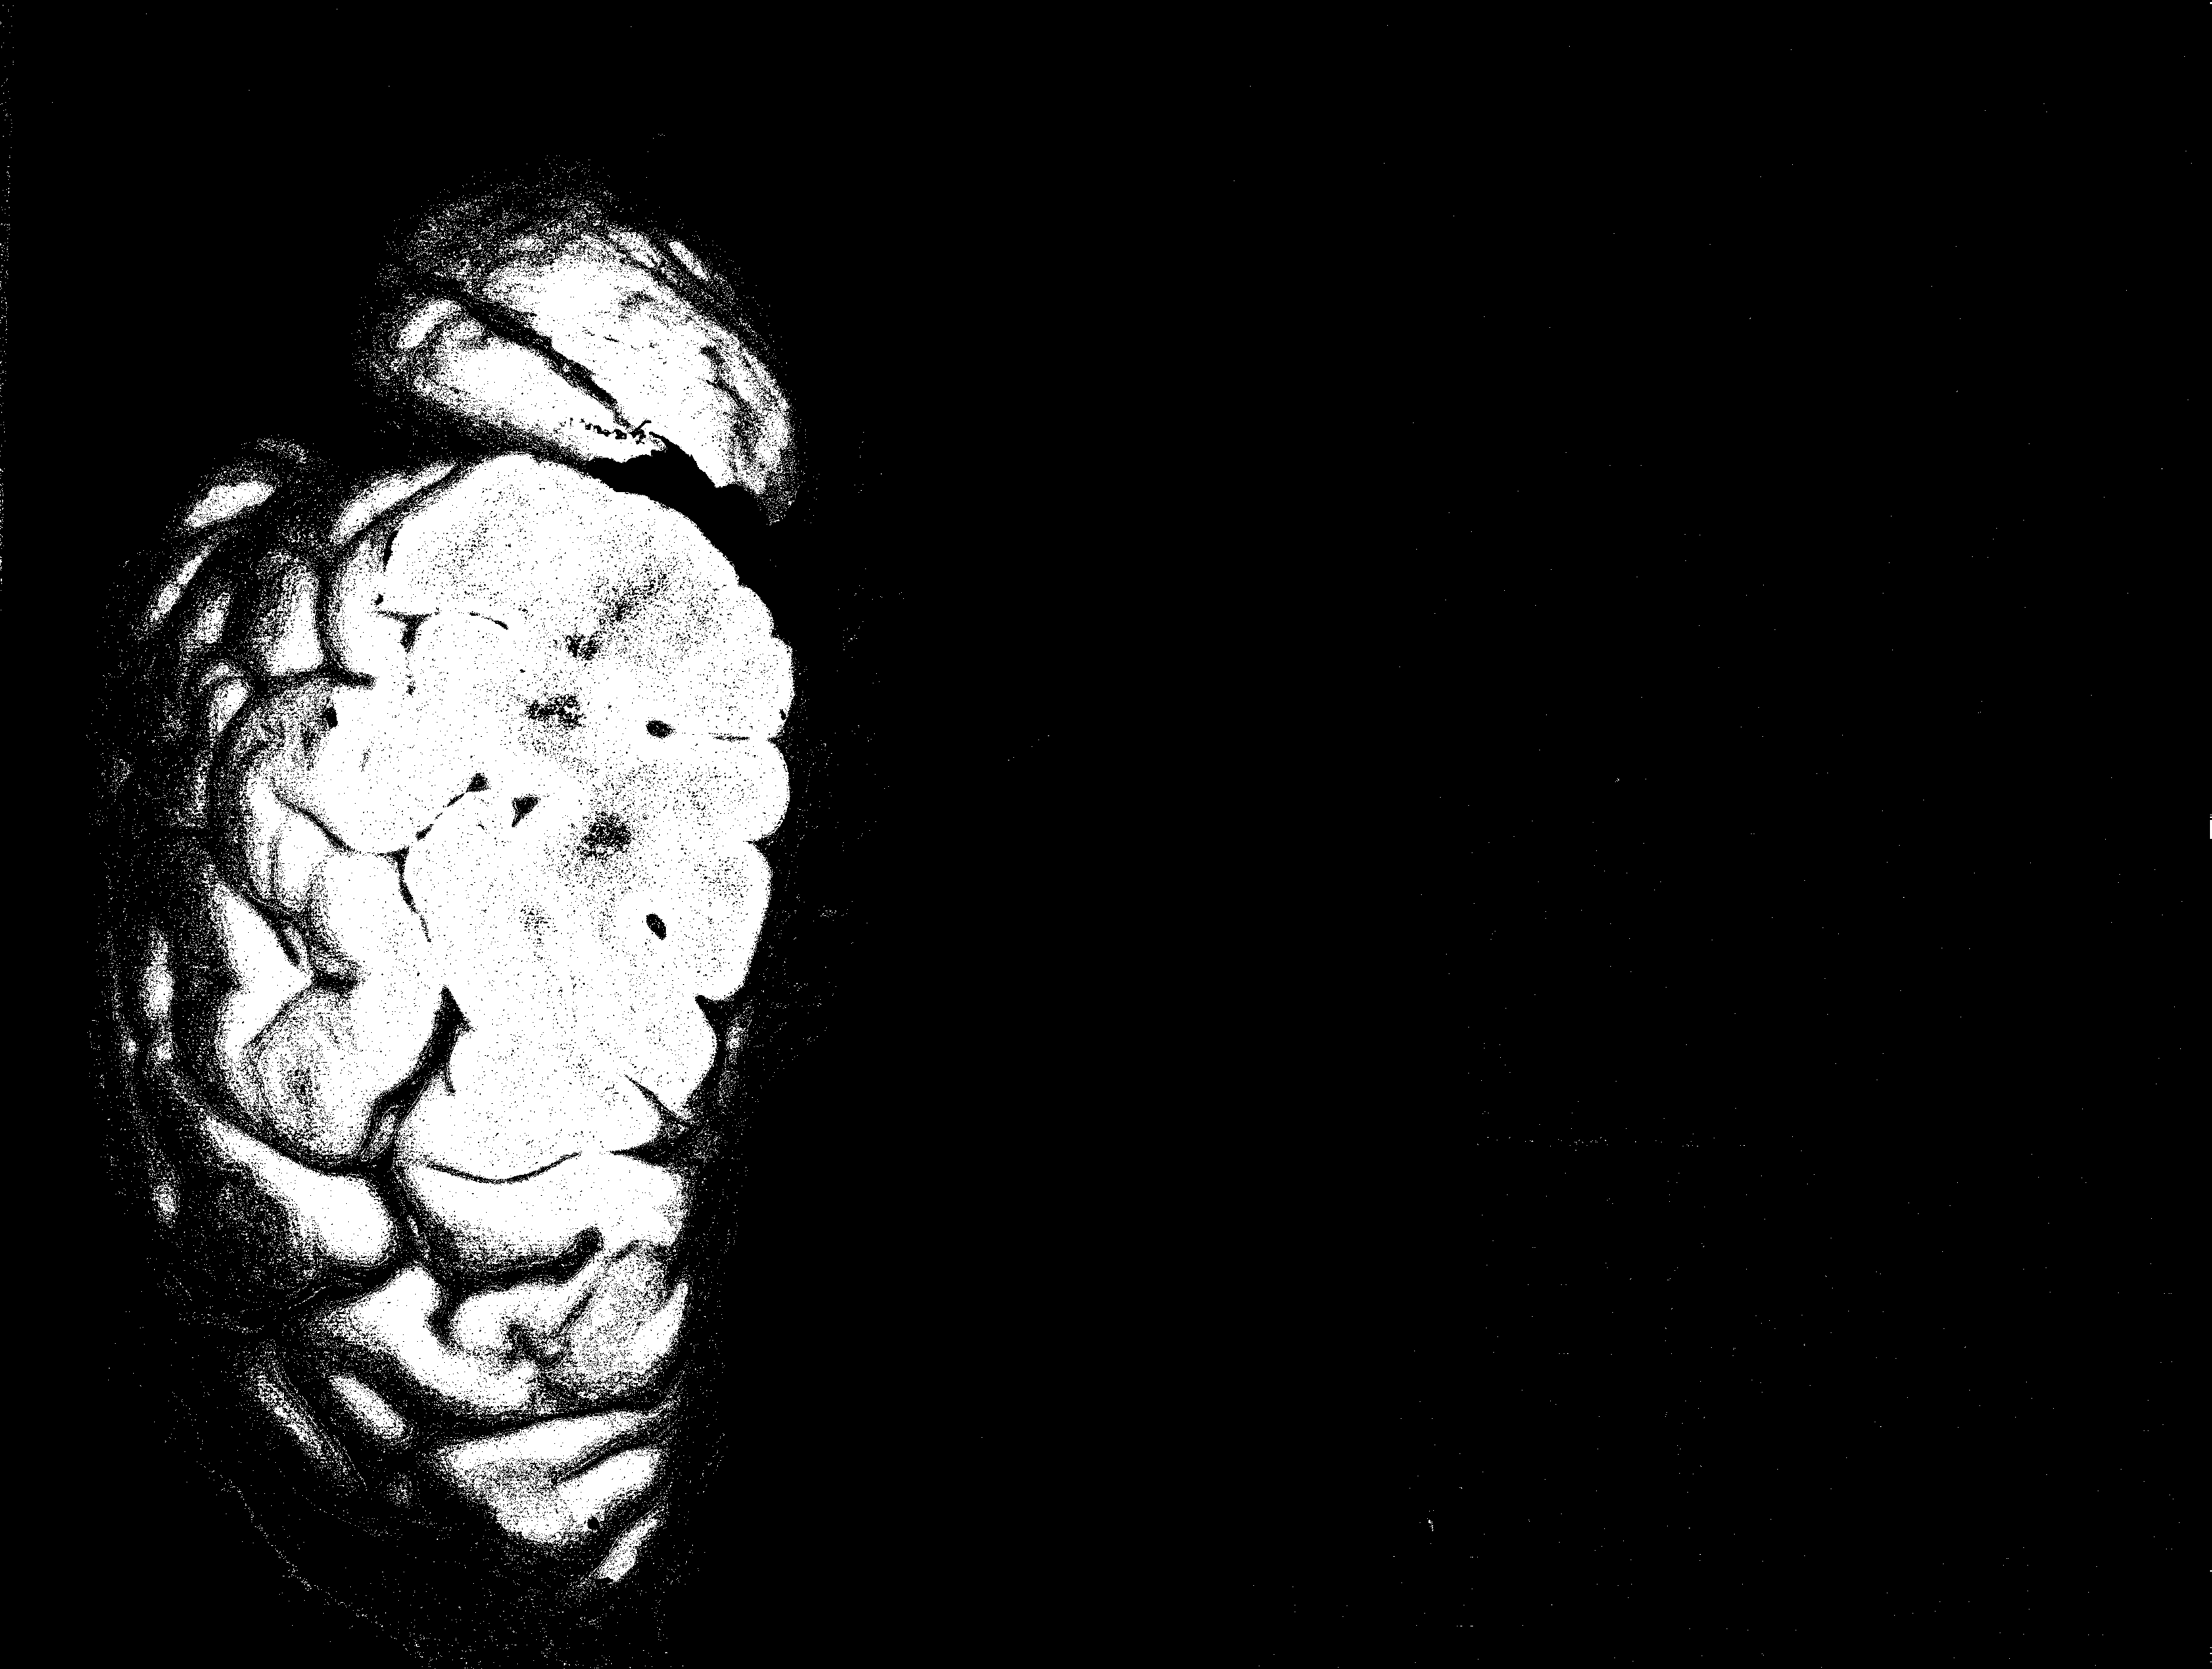
\includegraphics[width=0.7\linewidth]{graphics/predict200_svm_rbf} 
\caption{predicted image using svm with rbf kernel} 
\label{fig:predict200_svm_rbf} 
\end{figure}


\subsubsection{Local Features}

Despite adding the HSV color space, there is still no information
on the neighbourhood of a pixel. A first level approach to get information
on the neighbourhood of a pixel are statistical values like mean or
standard deviation. The statistical values are calculated on an $N\times N$
array around a pixel and assigned to the centered pixel. Figure \ref{calc_std}
shows how the standard deviation is calculated for an image. This
is done with the numpy and scipy modules. The \emph{generic\_filter}
function generates a window with the given size for every pixel and
calls the given function (e.g. numpy.std). 

\begin{figure}[H]


\begin{lstlisting}[language=Python,numbers=left]
def calc_std(img,size,use_mean=False):     
	"""Calculate the local standard deviation for each pixel of an image.
    Arguments:
        img : rgb image
        size : size of the window of neighbouring pixels
        use_mean : boolean, if False the standard deviation of R,G and B value are calculated and return as a 3 dimensional array.
                    if True the standard deviation of the mean is returned.
    Return:
      array_like, 3d or 2d
    """
    if not use_mean:
        std = np.zeros(img.shape)
        for i in range(img.shape[2]):
            std[:,:,i] = filters.generic_filter(img[:,:,i],np.std,size)
    else:
        mean_img = np.mean(img,axis=2)
        std = filters.generic_filter(mean_img,np.std,size)
    return std
\end{lstlisting}
\caption{Calculate the standard deviation using scipys generic\_filter method}
\label{calc_std}

\end{figure}



\subsubsection{Image Segmentation}


\subsection{Data Modeling}


\subsubsection{Support Vector Machines}

Support vector machines (SVMs) are one of the preferred classification
methods lately. They have a high accuracy, but their training time
is quite long. A model can easily be described by the found support
vectors.

SVMs can model nonlinear decision boundaries by using other kernels
instead of the linear kernel to increase the dimension of a vector.
A kernel defines the used scalar product. The most popular kernels
are the following:

\begin{itemize} 
\item linear:  $K(x,y) = \sum_{i=0}^n x_i\cdot y_i$ 
\item polynomial: $K(x,y) = (c+\sum_{i=0}^{n} x_i\cdot y_i)^d$	 	
\item rbf: $ \exp(-\frac{||x-y||^2}{2\sigma^2})$  
\end{itemize}  

\begin{figure}
\begin{tabular}{|l|r|r|r|}
\hline 	
Classifier 	& Accuracy & training time in s & test time in s \\  	
\hline 	
\hline 	
SVC (sklearn), rbf, 20k instances 	& 0.8752580408 	& 39.545465 	& 109.808209 	\\
\hline 	
\parbox[t]{6cm}{SVC (sklearn), rbf,\\ gamma=0.1, C=1, 20k instances} 	& 0.9579808675 	& 45.242423 	& 66.846724 \\  	
\hline 	
libSVM twister, 20k instances 	& 0.9592930497 	& 445.867 	& - \\  	
\hline 	
libSVM twister, 40k instances 	& 0.963317509 	& 934.912 	& - \\  	
\hline 	
libSVM twister, 100k instances 	& 0.9665214475 	& 3077.239 	& -\\ 	
\hline 
\end{tabular}  
\caption{SVMs from scikit-learn and Twister with rgb as features } 
\label{svm_table} 
\end{figure}

\begin{figure}
\begin{tabular}{|l|r|r|r|} 	
\hline 
Classifier & Accuracy & training time in s & test time in s \\  	
\hline 
GaussianNB & 0.9475908597 	& 0.042224 & 0.075098 \\  	
\hline 
Decision Tree & 0.9569552165 	& 0.563767 	& 0.057934 	\\  	
\hline 
RandomForest  & 0.9637635858 	& 1.698716 	& 0.399092 \\  	
\hline  
\end{tabular}  
\label{different_classifiers_table} 
\caption{Different classifiers used with rgb features.} 
\end{figure}

More information on SVMs can be found at \cite{Han2011}

\begin{figure} 
\centering 
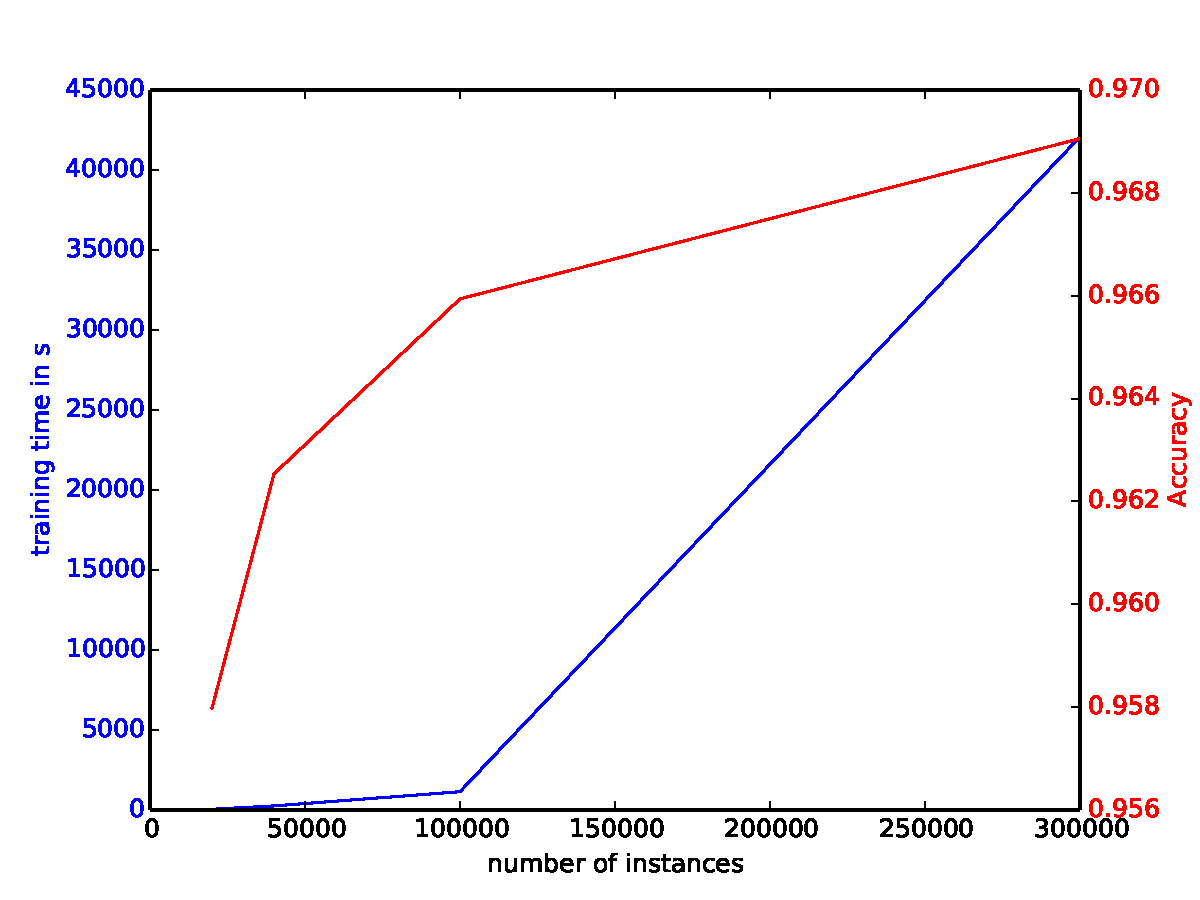
\includegraphics[width=0.8\linewidth]{graphics/sklearn_runtime} 
\caption{SVC training time with increasing sample} 
\label{fig:sklearn_runtime} 
\end{figure}


\subsection{Data Post Processing}


\subsection{Results}


